Este manual tiene como objetivo proporcionarte una guía detallada sobre cómo utilizar todas las características y funcionalidades de nuestra aplicación móvil.

\subsubsection{Requisitos del Sistema}
Antes de comenzar, asegúrate de que tu dispositivo cumple con los siguientes requisitos:

\begin{itemize}
	\item Sistema operativo móvil actualizado (recomendamos las últimas versiones de Android o iOS).
	\item Conexión a Internet estable.
\end{itemize}

\subsubsection{Acceso a la Aplicación}
Para acceder a nuestra aplicación móvil, sigue estos pasos:

\begin{enumerate}
	\item Abre la aplicación descargada en tu dispositivo.
	\item En la pantalla de inicio, puedes explorar las diferentes funcionalidades a través de la barra de navegación en la parte inferior.
\end{enumerate}

\subsubsection{Funcionalidades Principales}
A continuación, describiremos las funcionalidades principales de nuestra aplicación móvil:

\subsubsection{Registro de Usuario}
Para registrarte en nuestra aplicación, sigue estos pasos:

\begin{enumerate}
	\item Seleccione la opción “Cuenta” en la barra de navegación inferior.
	      Se abrirá un modal con campos para iniciar sesión y un enlace inferior en caso de no tener cuenta.
	      \begin{figure}[H]
		      \centering
		      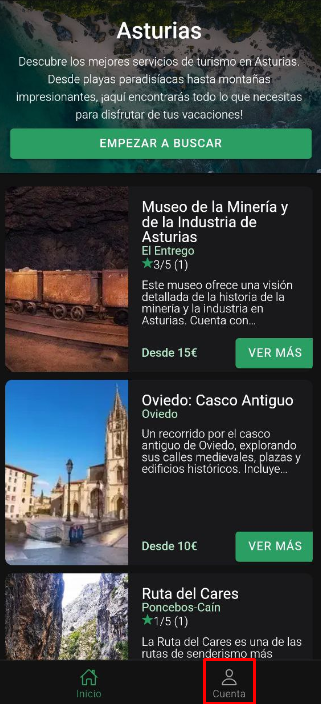
\includegraphics[width=0.3\textwidth]{7-Construccion/Manuales/app/P1-Registro.png}
		      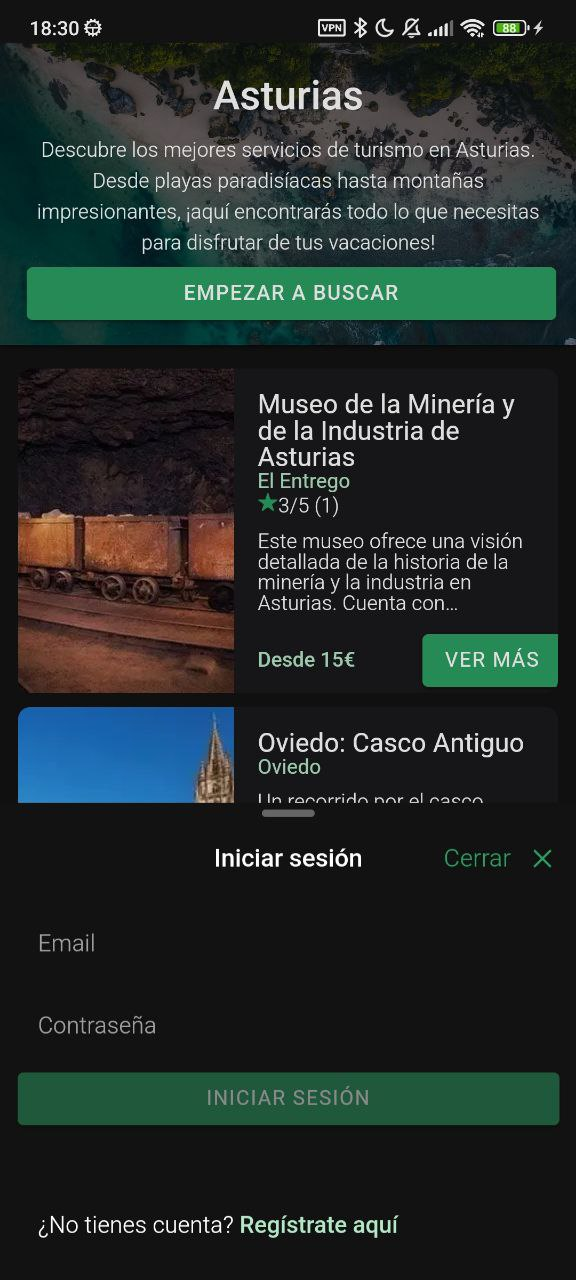
\includegraphics[width=0.3\textwidth]{7-Construccion/Manuales/app/inicio de sesion.png}
		      \caption{Registro - Indicación de donde está la opción “Cuenta” }
	      \end{figure}
	\item Haz clic en el enlace “Registrate aquí” para acceder al formulario de registro.
	      \begin{figure}[H]
		      \centering
		      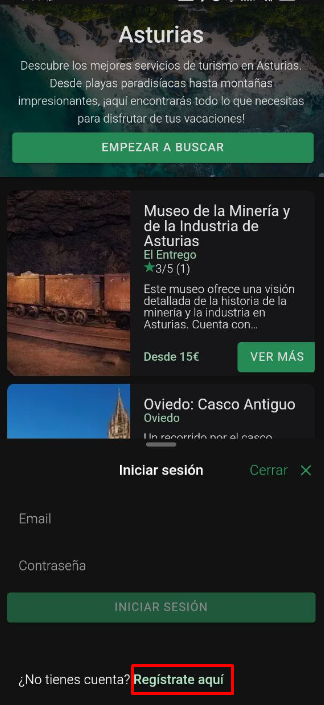
\includegraphics[width=0.3\textwidth]{7-Construccion/Manuales/app/P2-Registro.png}
		      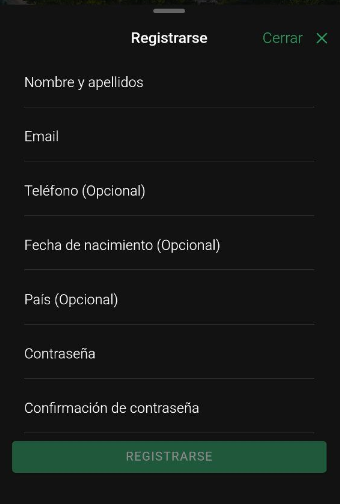
\includegraphics[width=0.3\textwidth]{7-Construccion/Manuales/app/registro.png}
		      \caption{Registro - Formulario de registro de usuario}
	      \end{figure}
	\item Completa el formulario de registro con tu información personal y pulsa el botón “Registrarse” para enviar el formulario.
\end{enumerate}

Al completar el registro con éxito, accederás automáticamente a tu cuenta y podrás comenzar a reservar actividades.

\subsubsection{Inicio de Sesión}
Si no tienes una cuenta, realiza el registro siguiendo los pasos descritos en la sección “Registro de Usuario” .
En cuanto la tengas, puedes iniciar sesión siguiendo estos pasos:

\begin{enumerate}
	\item Pulsa la pestaña “Cuenta” en la barra de navegación inferior. Se abrirá un modal con campos para iniciar sesión.
	      \begin{figure}[H]
		      \centering
		      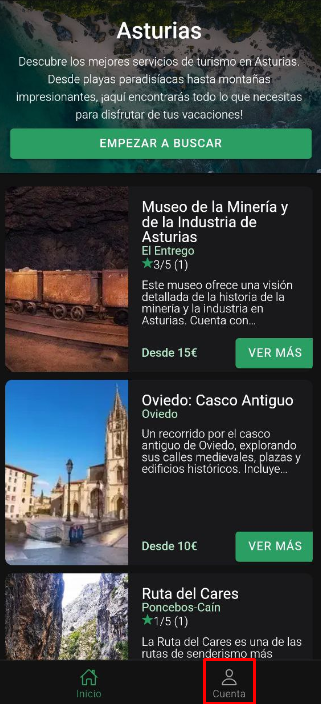
\includegraphics[width=0.3\textwidth]{7-Construccion/Manuales/app/P1-Registro.png}
		      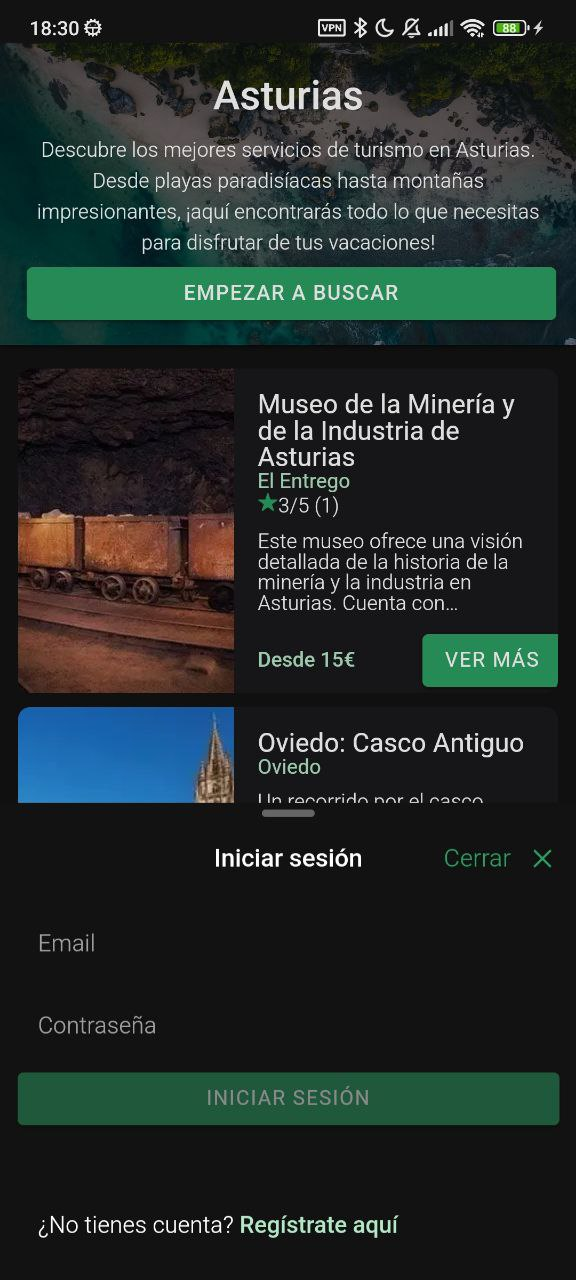
\includegraphics[width=0.3\textwidth]{7-Construccion/Manuales/app/inicio de sesion.png}
		      \caption{Inicio de sesion - Indicación de como acceder al formulario de inicio de sesión}
	      \end{figure}
	\item Ingresa tu email y contraseña en los campos correspondientes y pulsa el botón “Iniciar Sesión” para acceder a tu cuenta.
\end{enumerate}

Al iniciar sesión con éxito, accederás a tu cuenta y podrás comenzar a reservar actividades.

\subsubsection{Exploración de Actividades}
Desde la pantalla de inicio, puedes explorar las actividades pulsando la el botón “Empezar a buscar” . Te llevará a una página donde encontrarás una lista de actividades disponibles, con la opción de filtrar por nombre, por rango de fechas, precio máximo, número de personas, puntuación mínima e idioma.

\begin{figure}[H]
	\centering
	\includegraphics[width=0.3\textwidth]{7-Construccion/Manuales/app/P1-Exploración.png}
	\includegraphics[width=0.3\textwidth]{7-Construccion/Manuales/app/P2-Exploración.png}
	\caption{Redirección a la página de exploración de actividades y filtros de búsqueda}
\end{figure}

Para filtrar por nombre, ingresa el nombre de la actividad en la barra de búsqueda superior. A los 3 segundos de haber dejado de escribir, se mostrarán las actividades que coincidan con el nombre ingresado.
\begin{figure}[H]
	\centering
	\includegraphics[width=0.3\textwidth]{7-Construccion/Manuales/app/P3-Exploración.png}
	\caption{Campo de búsqueda de actividades}
\end{figure}

Para filtrar por una características más específicas, toca el botón “Filtros” que se encuentra en la parte superior derecha de la pantalla.
Se abrirá un menú con las opciones de filtrado disponibles.
\begin{figure}[H]
	\centering
	\includegraphics[width=0.3\textwidth]{7-Construccion/Manuales/app/P4-Exploración.png}
	\includegraphics[width=0.3\textwidth]{7-Construccion/Manuales/app/P5-Exploración.png}
	\caption{Abrir menú de filtros de búsqueda}
\end{figure}

Para filtrar por rango de fechas, selecciona las fechas de inicio y fin en los campos correspondientes.
\begin{figure}[H]
	\centering
	\includegraphics[width=0.3\textwidth]{7-Construccion/Manuales/app/P6-Exploración.png}
	\caption{Filtrar por rango de fechas}
\end{figure}

Para filtrar por precio máximo, ajusta el control deslizante.
\begin{figure}[H]
	\centering
	\includegraphics[width=0.3\textwidth]{7-Construccion/Manuales/app/P7-Exploración.png}
	\caption{Filtrar por precio máximo}
\end{figure}

Para filtrar por número de personas, utiliza los botones de incremento y decremento.
\begin{figure}[H]
	\centering
	\includegraphics[width=0.3\textwidth]{7-Construccion/Manuales/app/P8-Exploración.png}
	\caption{Filtrar por número de personas}
\end{figure}

Para filtrar por puntuación mínima, utiliza los botones de incremento y decremento.
\begin{figure}[H]
	\centering
	\includegraphics[width=0.3\textwidth]{7-Construccion/Manuales/app/P9-Exploración.png}
	\caption{Filtrar por puntuación mínima}
\end{figure}

Para filtrar por idioma, selecciona los idiomas deseados tocando las casillas correspondientes.
\begin{figure}[H]
	\centering
	\includegraphics[width=0.3\textwidth]{7-Construccion/Manuales/app/P10-Exploración.png}
	\caption{Filtrar por idioma}
\end{figure}

Para aplicar los filtros específicos, toca el botón “Añadir filtros” que se encuentra en la parte inferior de la pantalla.
En el caso que desees modificar los filtros aplicados, vuelve a pulsar el botón “Añadir filtros” después de haber seleccionado los filtros deseados.
\begin{figure}[H]
	\centering
	\includegraphics[width=0.3\textwidth]{7-Construccion/Manuales/app/P11-Exploración.png}
	\caption{Aplicar o modificar filtros adicionales}
\end{figure}

Una vez aplicados los filtros deseados, se mostrarán las actividades que coincidan con los filtros aplicados.
Y en caso de que desees hacer modificaciones o borrar los filtros, deberás pulsar el botón “Filtros aplicados (*)” que se encuentra en la parte inferior de la pantalla.
\begin{figure}[H]
	\centering
	\includegraphics[width=0.3\textwidth]{7-Construccion/Manuales/app/P12-Exploración.png}
	\caption{Ver filtros aplicados}
\end{figure}


Si deseas eliminar los filtros aplicados, toca el botón “Eliminar filtros” que se encuentra en la parte inferior de la pantalla
\begin{figure}[H]
	\centering
	\includegraphics[width=0.3\textwidth]{7-Construccion/Manuales/app/P13-Exploración.png}
	\caption{Eliminar filtros aplicados}
\end{figure}

\subsubsection{Ver Información Detallada de una Actividad}
Para ver la información detallada de una actividad, toca el botón “Ver más” de la actividad deseada.
Se abrirá una nueva pantalla con la información detallada de la actividad, incluyendo el nombre, la descripción, la duración, la puntuación y la ubicación.
\begin{figure}[H]
	\centering
	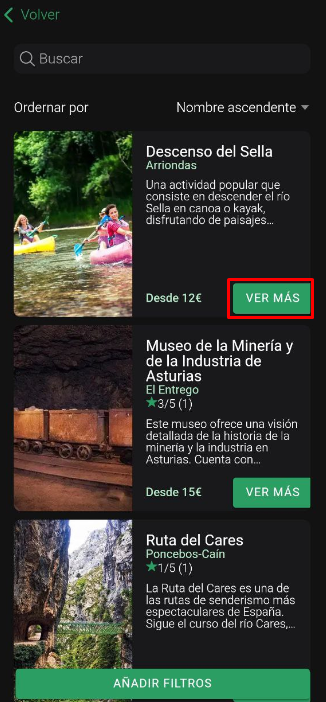
\includegraphics[width=0.3\textwidth]{7-Construccion/Manuales/app/P1-Actividad.png}
	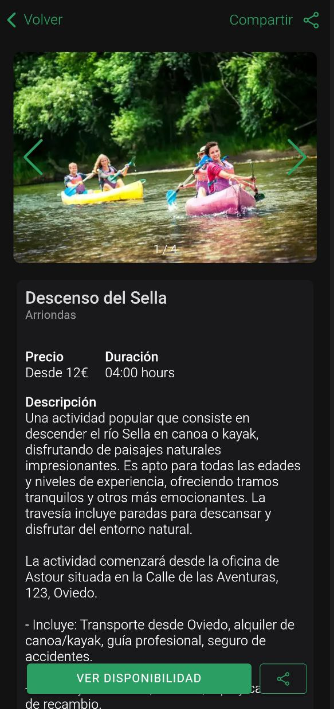
\includegraphics[width=0.3\textwidth]{7-Construccion/Manuales/app/P2-Actividad.png}
	\caption{Redirección a la página de información detallada de una actividad}
\end{figure}

Para ver los precios, idiomas y horarios de la actividad, toca el botón “Ver disponibilidad” que se encuentra en la parte inferior de la pantalla.
\begin{figure}[H]
	\centering
	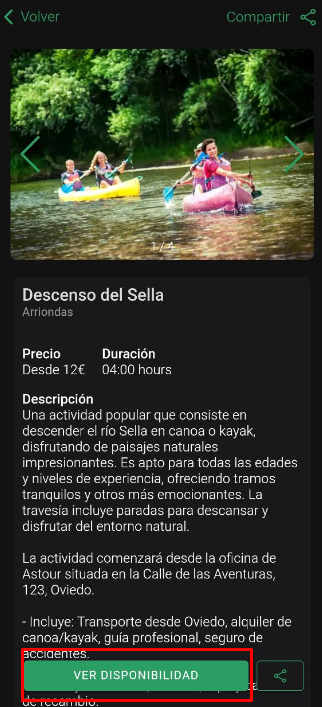
\includegraphics[width=0.3\textwidth]{7-Construccion/Manuales/app/P3-Actividad.png}
	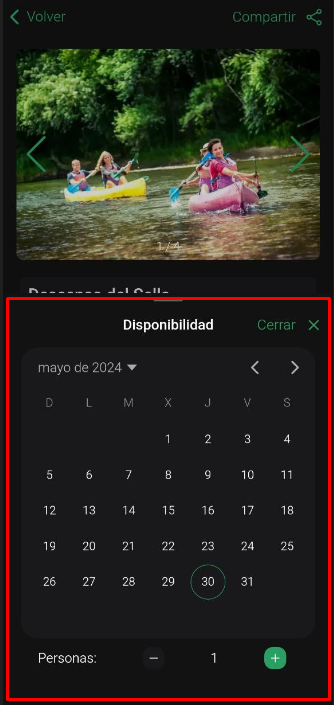
\includegraphics[width=0.3\textwidth]{7-Construccion/Manuales/app/P4-Actividad.png}
	\caption{Ver disponibilidad de una actividad}
\end{figure}

Desde esta pantalla podrás seleccionar la fecha en el calendario y el número de personas usando los botones de incremento y decremento.
Una vez seleccionada la fecha y el número de personas, podrás ver los precios, idiomas y horarios disponibles para la actividad.
\begin{figure}[H]
	\centering
	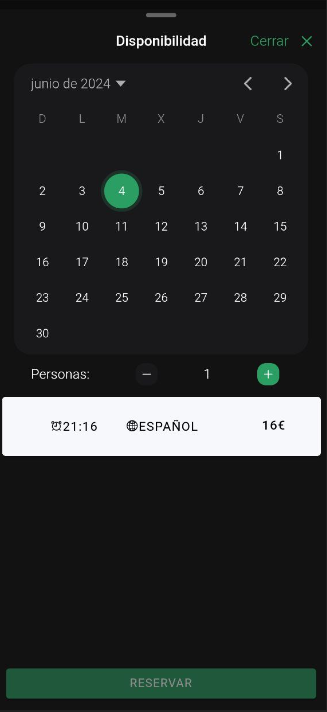
\includegraphics[width=0.3\textwidth]{7-Construccion/Manuales/app/P5-Actividad.png}
	\caption{Ver precios, idiomas y horarios de una actividad}
\end{figure}

\subsubsection{Reservar una Actividad}
Para reservar una actividad desde tu dispositivo móvil, sigue estos pasos:

\begin{enumerate}
	\item Sigue los pasos descritos en la sección “Ver Información Detallada de una Actividad” hasta ver la disponibilidad de la actividad.
	\item Selecciona la fecha en el calendario y el número de personas usando los botones de incremento y decremento.
	\item Selecciona el horario y el idioma deseados dentro de las opciones disponibles.
	\item Toca el botón “Reservar” para confirmar la reserva. Si no has iniciado sesión, se te pedirá que inicies sesión o te registres.
	      \begin{figure}[H]
		      \centering
		      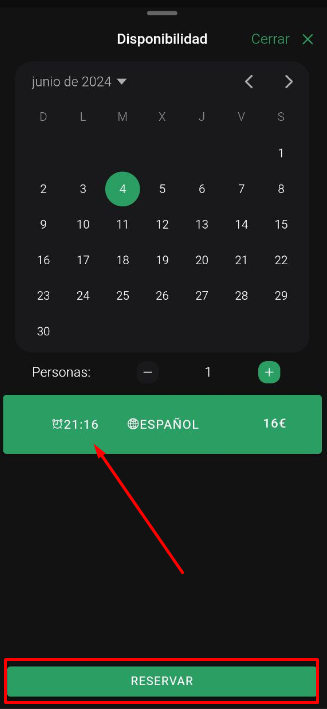
\includegraphics[width=0.3\textwidth]{7-Construccion/Manuales/app/P1-Reservar.png}
		      \caption{Botón de reserva de una actividad}
	      \end{figure}
	\item Se te llevará a una pantalla de confirmación de la reserva, donde verás tus datos personales (se pueden modificar si es necesario) y el precio total.
	      \begin{figure}[H]
		      \centering
		      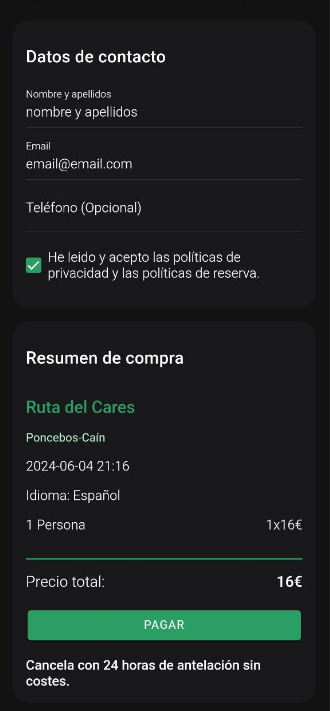
\includegraphics[width=0.3\textwidth]{7-Construccion/Manuales/app/P2-Reservar.png}
		      \caption{Pantalla de confirmación de reserva}
	      \end{figure}
	\item Toca el botón “Pagar” para poder rellenar el formulario con los datos de pago y así poder finalizar la reserva.
	      \begin{figure}[H]
		      \centering
		      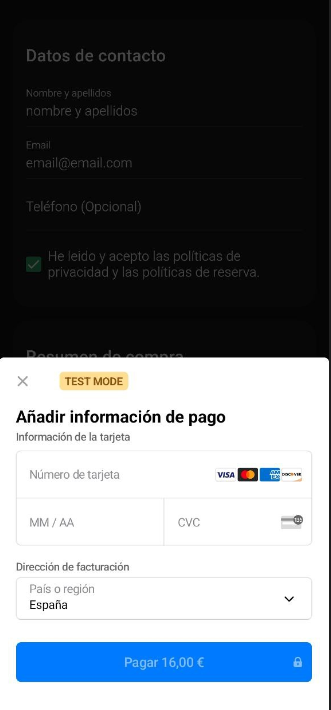
\includegraphics[width=0.3\textwidth]{7-Construccion/Manuales/app/P3-Reservar.png}
		      \caption{Pantalla de pago de reserva}
	      \end{figure}
	\item Una vez completado el formulario de pago, toca el botón “Pagar” para finalizar la reserva y recibir la confirmación de la misma.
	      \begin{figure}[H]
		      \centering
		      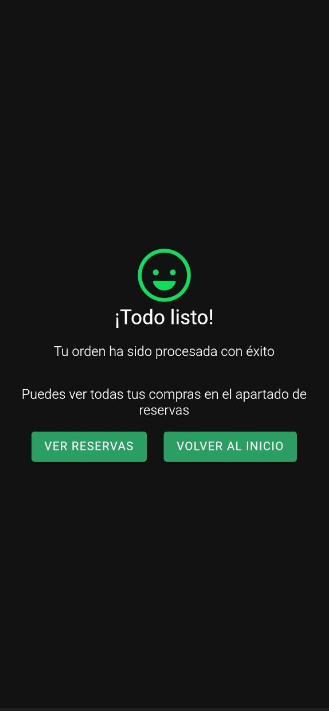
\includegraphics[width=0.3\textwidth]{7-Construccion/Manuales/app/P4-Reservar.png}
		      \caption{Confirmación de reserva}
	      \end{figure}
\end{enumerate}

\subsubsection{Gestión de Reservas}
Para gestionar tus reservas desde un dispositivo móvil, sigue estos pasos:
\begin{enumerate}
	\item Toca la pestaña “Reservas” en la barra de navegación inferior.
	      \begin{figure}[H]
		      \centering
		      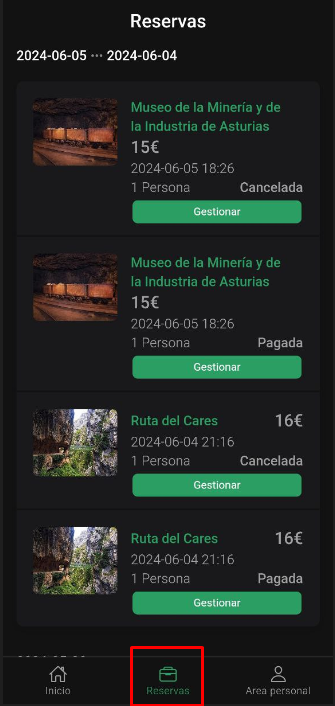
\includegraphics[width=0.3\textwidth]{7-Construccion/Manuales/app/P1-GestionReserva.png}
		      \caption{Indicación de donde está la opción “Reservas” }
	      \end{figure}
	\item Se abrirá una pantalla con un listado de tus reservas activas y pasadas.
	\item Para ver más detalles de una reserva, toca el botón “Gestionar” de la reserva deseada.
	      \begin{figure}[H]
		      \centering
		      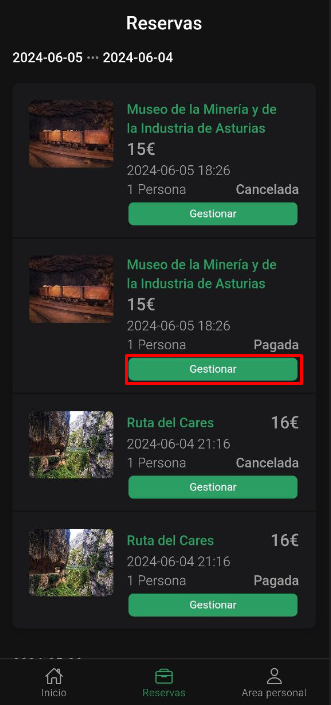
\includegraphics[width=0.3\textwidth]{7-Construccion/Manuales/app/P2-GestionReserva.png}
		      \caption{Botón de gestión de una reserva}
	      \end{figure}
	\item Se abrirá una nueva pantalla con la información detallada de la reserva, incluyendo la actividad, la fecha y hora, el idioma, el número de personas y el precio total.
	      \begin{figure}[H]
		      \centering
		      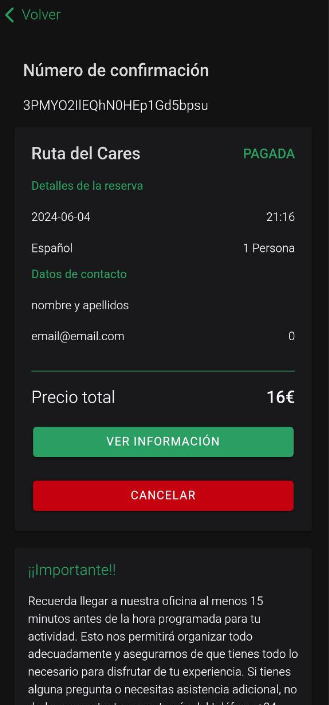
\includegraphics[width=0.3\textwidth]{7-Construccion/Manuales/app/P3-GestionReserva.png}
		      \caption{Información detallada de una reserva}
	      \end{figure}
	\item Para cancelar una reserva, toca el botón “Cancelar” de la reserva deseada.
	\item Se abrirá una pantalla de confirmación de la cancelación. Toca el botón “Confirmar” para cancelar la reserva.
\end{enumerate}

\subsubsection{Valoración}
Recuerda que puedes publicar una valoración de una actividad después de haberla realizado.

Para publicar una valoración de una actividad desde tu dispositivo móvil, sigue estos pasos:
\begin{enumerate}
	\item Toca la pestaña “Reservas” en la barra de navegación inferior.
	      \begin{figure}[H]
		      \centering
		      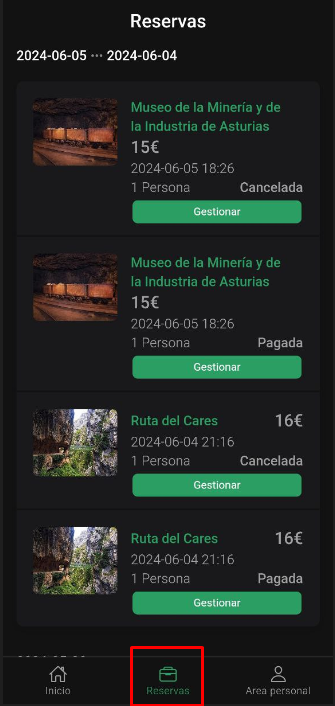
\includegraphics[width=0.3\textwidth]{7-Construccion/Manuales/app/P1-GestionReserva.png}
		      \caption{Indicación de donde está la opción “Reservas” }
	      \end{figure}
	\item Se abrirá una pantalla con un listado de tus reservas activas y pasadas.
	\item Toca el botón “Gestionar” de la reserva que deseas valorar.
	      \begin{figure}[H]
		      \centering
		      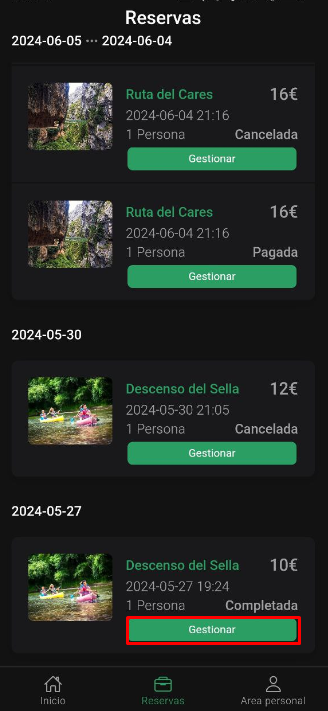
\includegraphics[width=0.3\textwidth]{7-Construccion/Manuales/app/P0-Publicar.png}
		      \caption{Botón de gestión de una reserva}
	      \end{figure}
	\item Se abrirá una nueva pantalla con la información detallada de la reserva, incluyendo la actividad, la fecha y hora, el idioma, el número de personas y el precio total.
	      \begin{figure}[H]
		      \centering
		      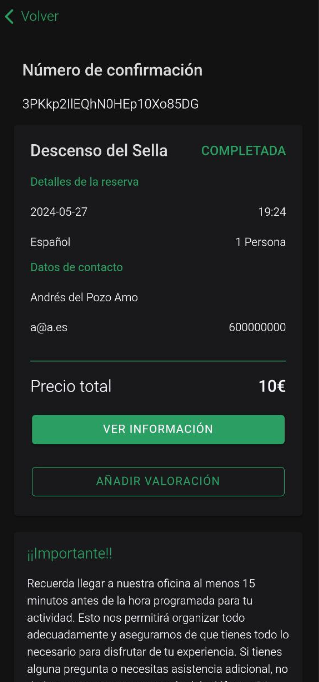
\includegraphics[width=0.3\textwidth]{7-Construccion/Manuales/app/P1-Publicar.png}
		      \caption{Información detallada de una reserva}
	      \end{figure}
	\item Para publicar una valoración, toca el botón “Añadir valoración” de la reserva deseada.
	      \begin{figure}[H]
		      \centering
		      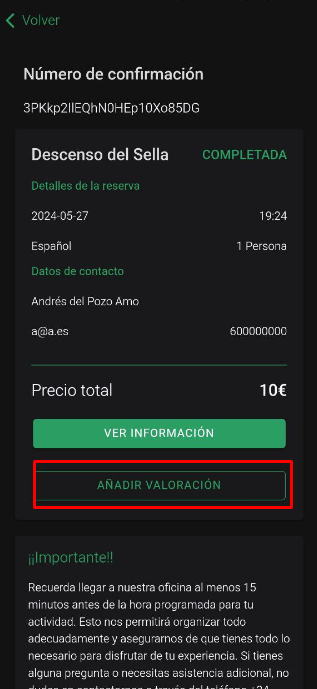
\includegraphics[width=0.3\textwidth]{7-Construccion/Manuales/app/P2-Publicar.png}
		      \caption{Botón de publicar valoración}
	      \end{figure}
	\item Se abrirá una nueva pantalla con un formulario para introducir tu puntuación y comentario (campo no obligatorio) de la actividad.
	      \begin{figure}[H]
		      \centering
		      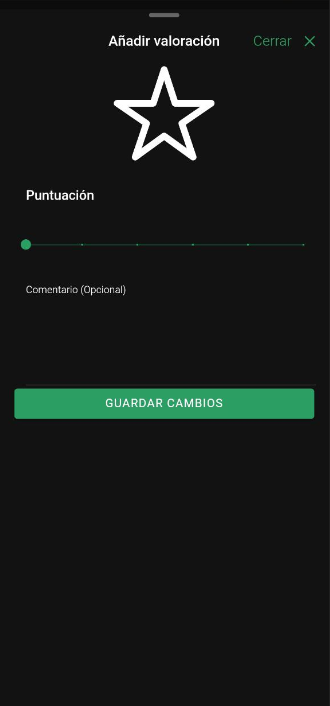
\includegraphics[width=0.3\textwidth]{7-Construccion/Manuales/app/P3-Publicar.png}
		      \caption{Formulario de publicar valoración}
	      \end{figure}
	\item Completa el formulario y toca el botón “Guardar cambios” para enviar la valoración.
	\item Al publicar la valoración con éxito, se mostrará el la valoración en la pantalla de la reserva.
	      \begin{figure}[H]
		      \centering
		      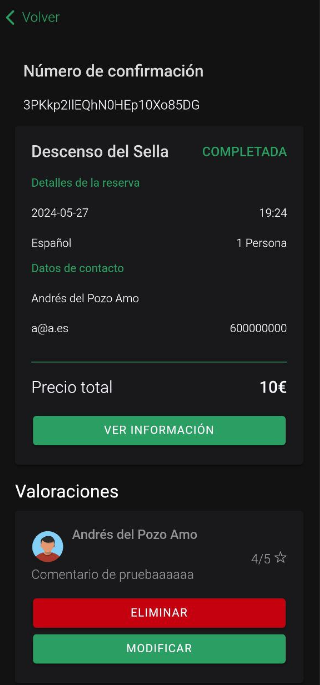
\includegraphics[width=0.3\textwidth]{7-Construccion/Manuales/app/P4-Publicar.png}
		      \caption{Reserva con valoración publicada}
	      \end{figure}

\end{enumerate}
Si deseas modificar la valoración, toca el botón “Modificar” de la reserva deseada.
\begin{figure}[H]
	\centering
	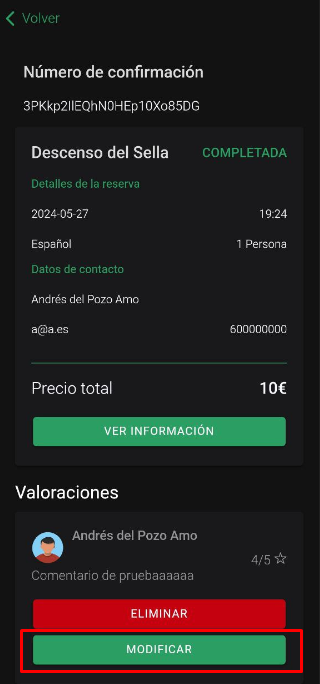
\includegraphics[width=0.3\textwidth]{7-Construccion/Manuales/app/P5-Publicar.png}
	\caption{Botón de modificar valoración}
\end{figure}
Si deseas eliminar la valoración, toca el botón “Eliminar” de la reserva deseada.
\begin{figure}[H]
	\centering
	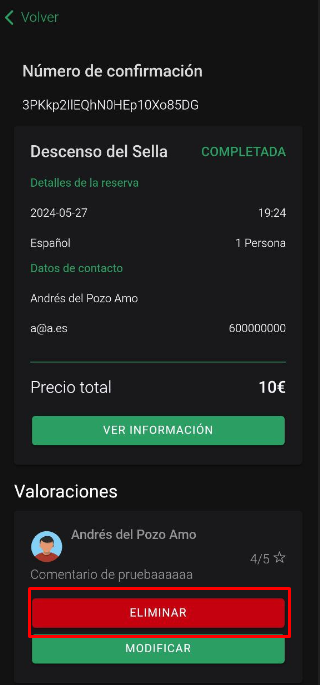
\includegraphics[width=0.3\textwidth]{7-Construccion/Manuales/app/P6-Publicar.png}
	\caption{Botón de eliminar valoración}
\end{figure}


\subsubsection{Cambiar Datos Personales}
Para cambiar tus datos personales desde tu dispositivo móvil, una vez hayas iniciado sesión, sigue estos pasos:
\begin{enumerate}
	\item Toca la pestaña “Área personal” en la barra de navegación inferior.
	      \begin{figure}[H]
		      \centering
		      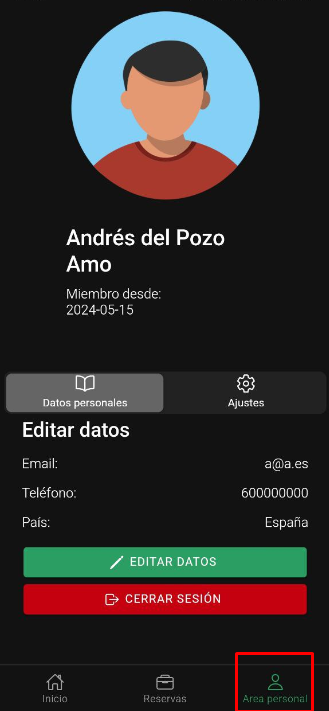
\includegraphics[width=0.3\textwidth]{7-Construccion/Manuales/app/P1-Perfil.png}
		      \caption{Indicación de donde está la opción “Área personal” }
	      \end{figure}
	\item Se abrirá una pantalla con tus datos personales y varios botones de acción.
	\item Toca el botón “Editar perfil” para acceder al formulario de edición de datos personales.
	      \begin{figure}[H]
		      \centering
		      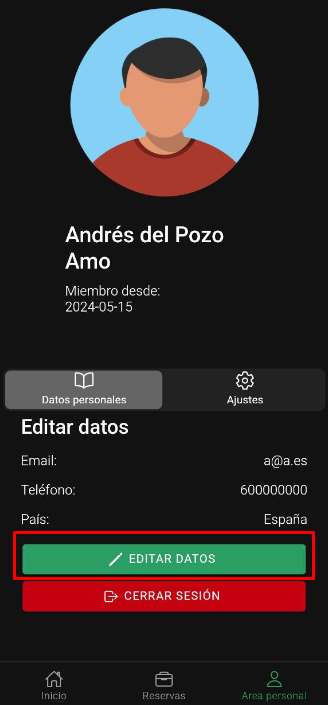
\includegraphics[width=0.3\textwidth]{7-Construccion/Manuales/app/P2-Perfil.png}
		      \caption{Botón de editar perfil}
	      \end{figure}
	\item Completa el formulario con los nuevos datos y toca el botón “Guardar cambios” para enviar el formulario.
	      \begin{figure}[H]
		      \centering
		      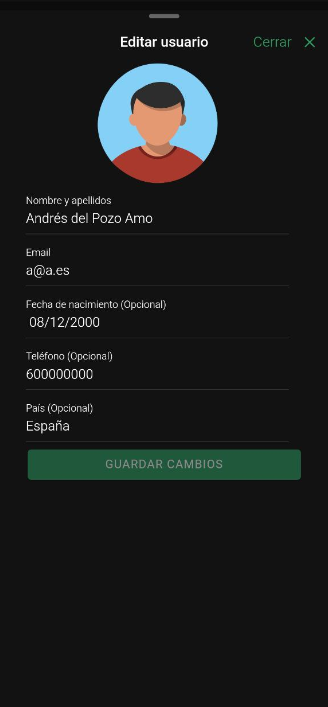
\includegraphics[width=0.3\textwidth]{7-Construccion/Manuales/app/P3-Perfil.png}
		      \caption{Formulario de edición de datos personales}
	      \end{figure}
	\item Para modificar la contraseña o eliminar la cuenta, toca la pestaña “Ajustes” dentro de la pantalla “Área personal”.
	      \begin{figure}[H]
		      \centering
		      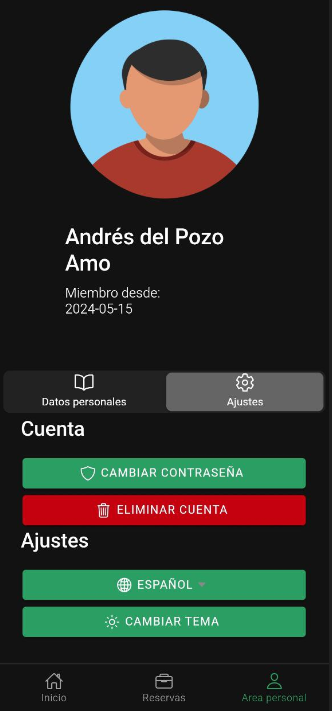
\includegraphics[width=0.3\textwidth]{7-Construccion/Manuales/app/P4-Perfil.png}
		      \caption{Pestaña de ajustes}
	      \end{figure}
	\item Toca el botón “Cambiar contraseña” para acceder al formulario de cambio de contraseña.
	      \begin{figure}[H]
		      \centering
		      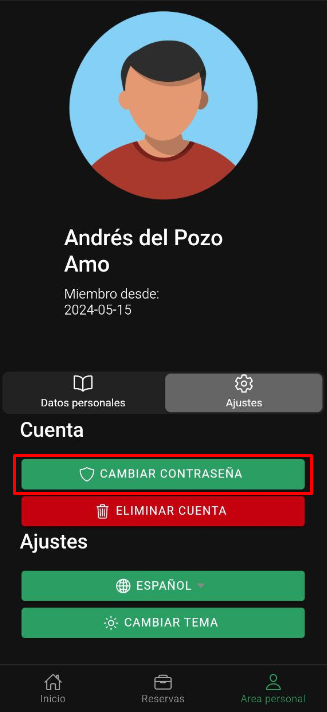
\includegraphics[width=0.3\textwidth]{7-Construccion/Manuales/app/P5-Perfil.png}
		      \caption{Botón de cambiar contraseña}
	      \end{figure}
	\item Completa el formulario con los nuevos datos y toca el botón “Guardar cambios” para enviar el formulario.
	      \begin {figure}[H]
	      \centering
	      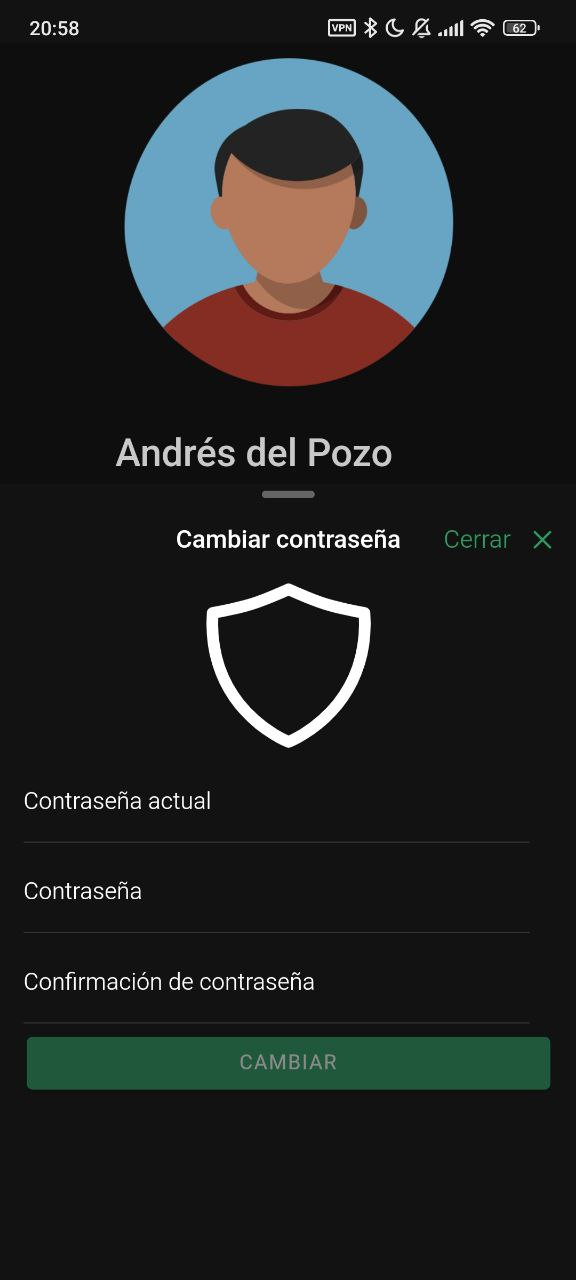
\includegraphics[width=0.3\textwidth]{7-Construccion/Manuales/app/P6-Perfil.png}
	      \caption{Formulario de cambio de contraseña}
	      \end{figure}
	\item Toca el botón “Eliminar cuenta” para eliminar tu cuenta de la aplicación.
	      \begin {figure}[H]
	      \centering
	      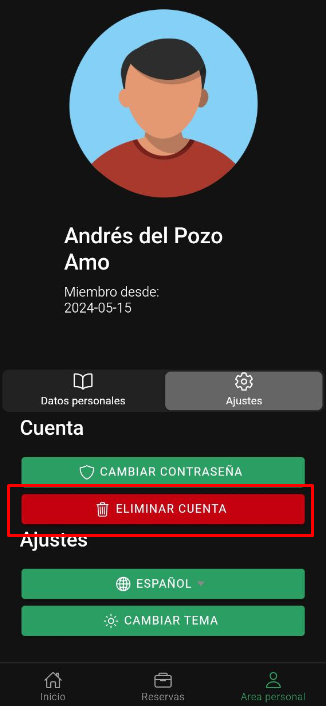
\includegraphics[width=0.3\textwidth]{7-Construccion/Manuales/app/P7-Perfil.png}
	      \caption{Botón de eliminar cuenta}
	      \end{figure}
	\item Se abrirá una pantalla de confirmación. Toca el botón “Confirmar” para eliminar tu cuenta.
\end{enumerate}

\subsubsection{Cerrar Sesión}
Para cerrar sesión desde tu dispositivo móvil, sigue estos pasos:
\begin{enumerate}
	\item Toca la pestaña “Área personal” en la barra de navegación inferior.
	      \begin{figure}[H]
		      \centering
		      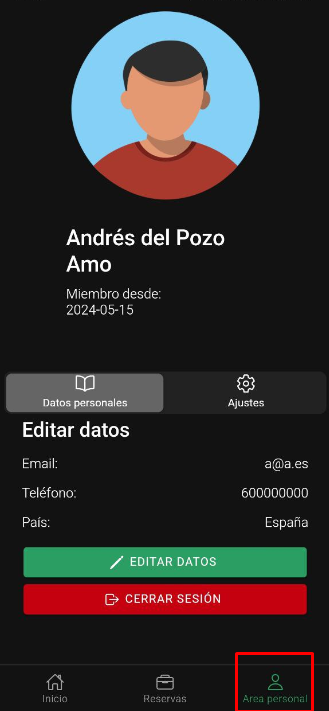
\includegraphics[width=0.3\textwidth]{7-Construccion/Manuales/app/P1-Perfil.png}
		      \caption{Indicación de donde está la opción “Área personal” }
	      \end{figure}
	\item Se abrirá una pantalla con tus datos personales y varios botones de acción.
	\item Toca el botón “Cerrar sesión” para salir de tu cuenta.
	      \begin{figure}[H]
		      \centering
		      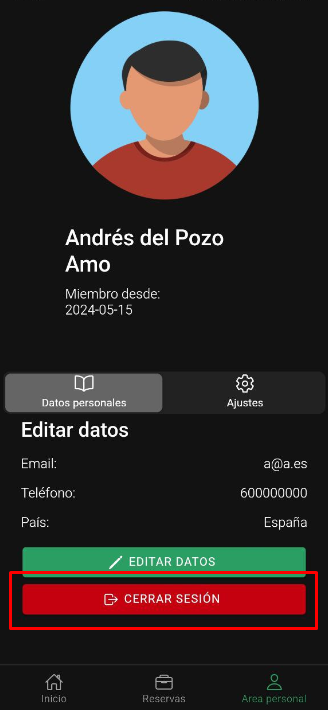
\includegraphics[width=0.3\textwidth]{7-Construccion/Manuales/app/P2-CerrarSesion.png}
		      \caption{Botón de cerrar sesión}
	      \end{figure}
	\item Se te redirigirá a la pantalla de inicio y habrás cerrado sesión con éxito.
\end{enumerate}
Si deseas volver a iniciar sesión, sigue los pasos descritos en la sección “Inicio de Sesión” .

\subsubsection{Cambiar Idioma}
Para cambiar el idioma de la aplicación desde tu dispositivo móvil, sigue estos pasos:
\begin{enumerate}
	\item Toca la pestaña “Área personal” en la barra de navegación inferior.
	      \begin{figure}[H]
		      \centering
		      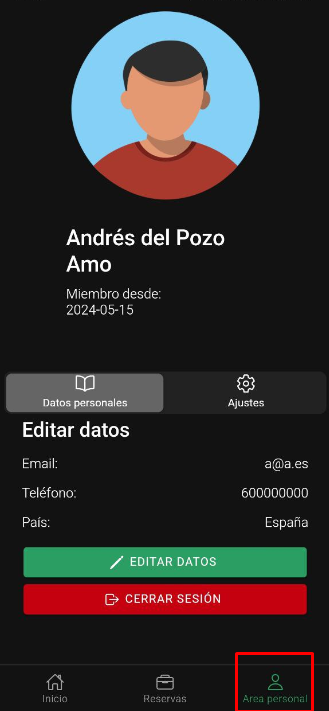
\includegraphics[width=0.3\textwidth]{7-Construccion/Manuales/app/P1-Perfil.png}
		      \caption{Indicación de donde está la opción “Área personal” }
	      \end{figure}
	\item Toca la pestaña “Ajustes” dentro de la pantalla “Área personal”.
	      \begin{figure}[H]
		      \centering
		      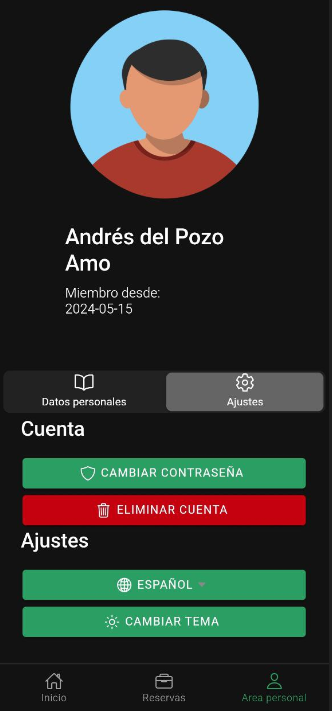
\includegraphics[width=0.3\textwidth]{7-Construccion/Manuales/app/P4-Perfil.png}
		      \caption{Pestaña de ajustes}
	      \end{figure}
	\item Toca la opción “Español” .
	      \begin{figure}[H]
		      \centering
		      \includegraphics[width=0.3\textwidth]{7-Construccion/Manuales/app/P5-Idioma.png}
		      \caption{Botón de idioma}
	      \end{figure}
	\item Se abrirá una lista de idiomas disponibles.
	\item Toca el idioma deseado para cambiar el idioma de la aplicación.
	\item La aplicación se actualizará automáticamente con el idioma seleccionado.
\end{enumerate}

\subsubsection{Cambiar Tema}
\begin{enumerate}
	\item Toca la pestaña “Área personal” en la barra de navegación inferior.
	      \begin{figure}[H]
		      \centering
		      \includegraphics[width=0.3\textwidth]{7-Construccion/Manuales/app/P1-Perfil.png}
		      \caption{Indicación de donde está la opción “Área personal” }
	      \end{figure}
	\item Toca la pestaña “Ajustes” dentro de la pantalla “Área personal”.
	      \begin{figure}[H]
		      \centering
		      \includegraphics[width=0.3\textwidth]{7-Construccion/Manuales/app/P4-Perfil.png}
		      \caption{Pestaña de ajustes}
	      \end{figure}
	\item Toca la opción “Cambiar tema” .
	      \begin{figure}[H]
		      \centering
		      \includegraphics[width=0.3\textwidth]{7-Construccion/Manuales/app/P5-Tema.png}
		      \caption{Botón de tema}
	      \end{figure}

	\item La aplicación se actualizará automáticamente con el tema contrario. Si el tema actual es claro, se cambiará a oscuro y viceversa.
	\item El icono de la opción de tema cambiará al tema contrario. Si el tema actual es claro, se cambiará a una luna y si el tema actual es oscuro, se cambiará a un sol.
\end{enumerate}

\subsubsection{Soporte Técnico}
Si encuentras algún problema o tienes alguna pregunta relacionada con el uso de nuestra aplicación, no dudes en contactar a nuestro equipo de soporte técnico.
Puedes encontrar la información de contacto en el apartado “Ajustes” en la sección de “Área personal” de la aplicación, pulsando el icono de información en la parte superior derecha de la pantalla.
\begin{figure}[H]
	\centering
	\includegraphics[width=0.3\textwidth]{7-Construccion/Manuales/app/P1-Info.png}
	\includegraphics[width=0.3\textwidth]{7-Construccion/Manuales/app/P2-Info.png}
	\caption{Icono e información de contacto}
\end{figure}
